\documentclass[10pt,a4paper]{article}
\usepackage{amsmath}
\usepackage{amsfonts}
\usepackage{amssymb}
\usepackage{graphicx}
\usepackage[T1]{fontenc}
\usepackage[utf8]{inputenc}

\title{Grenouille}
\date {14 décembre 2018}
\author{Groupe Introduction à \LaTeX}


\begin{document}
% Let's have fun with github \o/



	\maketitle

	\section{Grenouilles dans la culture}
\subsection{Mythes bibliques}
Les grenouilles sont parfois présentes dans d'étranges phénomènes : les pluies d'animaux.

Dans la Bible, la deuxième des dix plaies d'Égypte est l'invasion des terres par des milliers de ces batraciens. 
D'après les scientifiques qui se sont penchés sur cet évènement, le phénomène pourrait s'expliquer par une sécheresse ou par l'empoisonnement des eaux du Nil.
 En effet, dans des situations de stress, ces animaux sont capables d'accélérer leur développement pour fuir plus vite leur milieu, d'où une explosion de leur nombre.

De ce fait, on peut lire dans la bible de nombreuses références négatives sur les grenouilles.
\subsubsection{Exode}
\begin{itemize}
\item 7 - 27 : Si tu refuses, toi, de le laisser partir, moi je vais infester de grenouilles tout ton territoire.
\item 7 - 28 : Le Fleuve grouillera de grenouilles, elles monteront et entreront dans ta maison, dans la chambre où tu couches, sur ton lit, dans les maisons de tes serviteurs et de ton peuple, dans tes fours et dans tes huches.
\item 7 - 29 : Les grenouilles grimperont même sur toi, sur ton peuple et sur tous tes serviteurs.
\item 8 - 1 : Yahvé dit à Moïse : Dis à Aaron : Étends ta main avec ton bâton sur les fleuves, les canaux et les marais, et fais monter les grenouilles sur la terre d'Égypte.
\item 8 - 2 : Aaron étendit la main sur les eaux d'Égypte, les grenouilles montèrent et recouvrirent la terre d'Égypte.
\item 8 - 3 : Mais les magiciens avec leurs sortilèges en firent autant, et firent monter les grenouilles sur la terre d'Égypte.
\item 8 - 4 : Pharaon appela Moïse et Aaron et dit : Priez Yahvé de détourner les grenouilles de moi et de mon peuple, et je m'engage à laisser partir le peuple pour qu'il sacrifie à Yahvé.
\item 8 - 5 : Moïse dit à Pharaon : À toi l'avantage! Pour quand dois-je prier pour toi, pour tes serviteurs et pour ton peuple, afin que les grenouilles soient supprimées de chez toi et de vos maisons pour ne rester que dans le Fleuve?
\item 8 - 7 : Les grenouilles s'éloigneront de toi, de tes maisons, de tes serviteurs, de ton peuple, et il n'en restera plus que dans le Fleuve.
\item 8 - 8 : Moïse et Aaron sortirent de chez Pharaon, et Moïse cria vers Yahvé au sujet des grenouilles qu'il avait infligées à Pharaon.
\item 8 - 9 : Yahvé fit ce que demandait Moïse, et les grenouilles crevèrent dans les maisons, dans les cours et dans les champs.
\end{itemize}
\subsubsection{Psaumes}
\begin{itemize}
\item 78 - 45 : Il leur envoya des taons qui dévoraient, des grenouilles qui les infestaient.
\item 105 - 30 : Leur pays grouilla de grenouilles jusque dans les chambres des rois.
\end{itemize}
\subsubsection{Sagesse}
\begin{itemize}
\item 19 - 10 : Ils se souvenaient encore des événements de leur exil, comment la terre, et non des animaux, avait produit des moustiques, et comment le Fleuve, et non des êtres aquatiques, avait vomi une multitude de grenouilles.
\end{itemize}
\subsection{L'Apocalypse}
\begin{itemize}
\item 16 - 13 : Puis, de la gueule du Dragon, et de la gueule de la Bête, et de la gueule du faux prophète, je vis surgir trois esprits impurs, comme des grenouilles.
\end{itemize}
\subsection{Autres mythes}
\subsubsection{Grenouille météorologue}
\subsection{Allégorie}

	
	\include{Voiraussi/Voirsaussi}
	

\section{Étymologie et nomenclature}

La racine du mot $\ll$ grenouille $\gg$ vient du latin rana, voulant dire grenouille, et ranucula ou ranunculus, petite grenouille. Utilisé dès l'époque médiévale sous sa forme ancienne $\ll$ renoille $\gg$ ou $\ll$ grenoille $\gg$ au XIIIe siècle, le mot $\ll$ grenouille $\gg$ est attesté à partir du début du XVIe siècle. Le $\ll$ g $\gg$ initial ayant sans doute été ajouté par évocation du cri guttural de ces animaux2.

Le mot $\ll$ grenouille $\gg$ est déjà présent dans les dictionnaires de français anciens en 1606. Dès sa première édition, en 1694, le Dictionnaire de L'Académie française en donne une définition surprenante : $\ll$ Insecte (sic) qui vit ordinairement dans les marais $\gg$. Insecte est corrigé en $\ll$ petit animal $\gg$ dans la quatrième édition de 1762 avec comme précision $\ll$ quadrupède et ovipare $\gg$ dans sa sixième édition. Il faut attendre la huitième édition de 1932 pour que la grenouille soit mentionnée comme appartenant à $\ll$ l'ordre des Batraciens $\gg$ (désormais ordre des amphibiens)3.

Diderot et d'Alembert, dans l' Encyclopédie ou Dictionnaire raisonné des sciences, des arts et des métiers (1751 à 1772) décrivent d'abord la grenouille comme un $\ll$ animal qui a quatre piés, qui respire par des poumons, qui n'a qu'un ventricule dans le cœur, \& qui est ovipare $\gg$, en distinguant les grenouilles aquatiques des rainettes arboricoles4.

La grenouille coasse. Il ne faut pas confondre avec le cri du corbeau qui croasse.

Une grenouillette est une petite grenouille5.

La larve de la grenouille s'appelle un têtard.

Parmi les amphibiens, on distinguait autrefois spontanément les crapauds des grenouilles, nom donné à d'autres espèces d'anoures, les premiers étaient caractérisés par une peau plus rugueuse, voire pustuleuse, un œil à pupille horizontale, un museau arrondi6, des pattes plus courtes, une moindre capacité à sauter, une marche plus lente, et le fait qu'ils passent moins de temps dans le milieu aquatique que les grenouilles7. Toutes les langues n'utilisent pas des dénominations particulières pour désigner les espèces d'anoures appelées en français sonneur, grenouille, rainette et crapaud. Certaines langues peuvent faire une distinction analogues comme l'anglais avec toad et frog, mais il n'y a pas forcément de correspondance pour une espèce, autrement dit il est abusif de traduire systématiquement frog par grenouille. 	
\section{Grenouilles dans la culture}
\subsection{Mythes bibliques}
Les grenouilles sont parfois présentes dans d'étranges phénomènes : les pluies d'animaux.

Dans la Bible, la deuxième des dix plaies d'Égypte est l'invasion des terres par des milliers de ces batraciens. 
D'après les scientifiques qui se sont penchés sur cet évènement, le phénomène pourrait s'expliquer par une sécheresse ou par l'empoisonnement des eaux du Nil.
 En effet, dans des situations de stress, ces animaux sont capables d'accélérer leur développement pour fuir plus vite leur milieu, d'où une explosion de leur nombre.

De ce fait, on peut lire dans la bible de nombreuses références négatives sur les grenouilles.
\subsubsection{Exode}
\begin{itemize}
\item 7 - 27 : Si tu refuses, toi, de le laisser partir, moi je vais infester de grenouilles tout ton territoire.
\item 7 - 28 : Le Fleuve grouillera de grenouilles, elles monteront et entreront dans ta maison, dans la chambre où tu couches, sur ton lit, dans les maisons de tes serviteurs et de ton peuple, dans tes fours et dans tes huches.
\item 7 - 29 : Les grenouilles grimperont même sur toi, sur ton peuple et sur tous tes serviteurs.
\item 8 - 1 : Yahvé dit à Moïse : Dis à Aaron : Étends ta main avec ton bâton sur les fleuves, les canaux et les marais, et fais monter les grenouilles sur la terre d'Égypte.
\item 8 - 2 : Aaron étendit la main sur les eaux d'Égypte, les grenouilles montèrent et recouvrirent la terre d'Égypte.
\item 8 - 3 : Mais les magiciens avec leurs sortilèges en firent autant, et firent monter les grenouilles sur la terre d'Égypte.
\item 8 - 4 : Pharaon appela Moïse et Aaron et dit : Priez Yahvé de détourner les grenouilles de moi et de mon peuple, et je m'engage à laisser partir le peuple pour qu'il sacrifie à Yahvé.
\item 8 - 5 : Moïse dit à Pharaon : À toi l'avantage! Pour quand dois-je prier pour toi, pour tes serviteurs et pour ton peuple, afin que les grenouilles soient supprimées de chez toi et de vos maisons pour ne rester que dans le Fleuve?
\item 8 - 7 : Les grenouilles s'éloigneront de toi, de tes maisons, de tes serviteurs, de ton peuple, et il n'en restera plus que dans le Fleuve.
\item 8 - 8 : Moïse et Aaron sortirent de chez Pharaon, et Moïse cria vers Yahvé au sujet des grenouilles qu'il avait infligées à Pharaon.
\item 8 - 9 : Yahvé fit ce que demandait Moïse, et les grenouilles crevèrent dans les maisons, dans les cours et dans les champs.
\end{itemize}
\subsubsection{Psaumes}
\begin{itemize}
\item 78 - 45 : Il leur envoya des taons qui dévoraient, des grenouilles qui les infestaient.
\item 105 - 30 : Leur pays grouilla de grenouilles jusque dans les chambres des rois.
\end{itemize}
\subsubsection{Sagesse}
\begin{itemize}
\item 19 - 10 : Ils se souvenaient encore des événements de leur exil, comment la terre, et non des animaux, avait produit des moustiques, et comment le Fleuve, et non des êtres aquatiques, avait vomi une multitude de grenouilles.
\end{itemize}
\subsection{L'Apocalypse}
\begin{itemize}
\item 16 - 13 : Puis, de la gueule du Dragon, et de la gueule de la Bête, et de la gueule du faux prophète, je vis surgir trois esprits impurs, comme des grenouilles.
\end{itemize}
\subsection{Autres mythes}
\subsubsection{Grenouille météorologue}
\subsection{Allégorie}




\include{Voiraussi/Voirsaussi}

	\section{La reproduction des battraciens}



\subsection{La différenciation mâle/femelle}

Si le sexe est déterminé génétiquement, il est modulé par les conditions thermiques. 
Si l’hiver a été doux et bref, la production d’individus hermaphrodites augmente dans la population.
La différenciation sexuelle est postérieure à la métamorphose et a lieu lors de la croissance.
Le mâle possède une taille légèrement plus petite que la femelle.
La maturité sexuelle est acquise plus ou moins tardivement (en 3 ans pour la grenouille rousse). 
A partir de ce stade, en théorie, la croissance se poursuit lentement et indéfiniment. La grenouille vit en moyenne 5 ans, sa longévité maximale est de 15 ans.
        
\subsection{Le choix du partenaire}

En mars, les grenouilles sortent de leur hibernation.  
Dès que la température extérieure atteint environ 7deg C, les individus se mettent en route vers le site de reproduction, s’il n’était pas déjà sur place. 
Chez la plupart des espèces, l’accouplement a lieu dans l’eau.

Les femelles, encore à quelques kilomètres de distance, perçoivent le cri nuptial émis par leurs congénères grâce aux gonflements des sacs vocaux.


\begin{figure}
	\begin{center}
<<<<<<< HEAD
		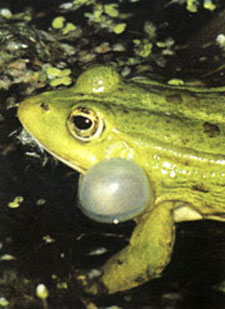
\includegraphics[width=.5\textwidth]{laRepro/sacvocal.jpg}
		\caption{Gonflement des sacs vocaux permettant l'émission de son.}%
		\label{fig:grossejoue}
	\end{center}
=======

	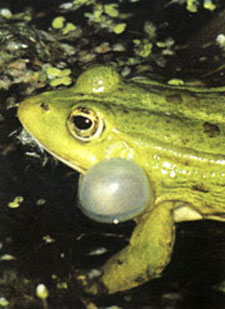
\includegraphics[width=.5\textwidth]{laRepro/sacvocal.jpg}	
	\end{center}
	\caption{Gonflement des sacs vocaux permettant l'émission de son.}%
	\label{fig:grossejoue}
>>>>>>> 9c1c91cf300d3ed68f23f2e076351a9ee57079a7
\end{figure}

Lorsque les femelles rejoignent le lieu d’accouplement, plusieurs mâles (parfois plus de 6) s’assemblent autour de chaque femelle. 
Dans certains cas, la qualité des vocalisations du mâle détermine le choix fait par la femelle. Cela est dangereux car cela peut attirer des prédateurs.

La femelle, reconnue avant tout par les phéromones qu’elle produit, est saisie par le mâle, qui glisse les bras sous ses aisselles. 
Pouce et avant-bras portent des callosités, les brosses copulatrices dont l’apparition (et la disparition après la reproduction) est contrôlée par les variations de sécrétion d’une hormone, la testostérone.
Le contact des brosses sur la peau de la femelle suscite un réflexe d’étreinte, soudant littéralement les deux partenaires. 
L’étreinte peut durer 7 jours ou plus. Les oeufs, expulsés du cloaque de la femelle, sont fécondés de manière externe par le mâle. La ponte finie, mâle et femelle se séparent.

 
\subsection{La ponte}

Les grenouilles européennes pondent de 1400 à 10 000 oeufs, d’un diamètre compris entre 1 et 3 mm. 
Chez certaines grenouilles américaines et tropicales, leur nombre peut dépasser 20 000 et le diamètre atteint 5 mm. 
Dotés d’un vitallus assez important, ils s’agglomèrent en de volumineuses masses gélatineuses.

Certaines grenouilles sont vivipares. 
Elles avalent alors leurs oeufs fécondés afin de les faire incuber dans l’estomac. 
Elles accouchent ensuite de petites grenouilles par la bouche. 
L’inhibition gastrique maintenue pendant toute la " gestation " est alors levée.

Cependant l’oviparité est le mode de reproduction le plus répandu. 
Chez certaines espèces, quand les oeufs sont en train d’éclore, le mâle se place au milieu, s’enduit de la gelée de la ponte et entre dans une torpeur progressive, pendant laquelle les têtards éclos sautent afin d’escalader son corps ; ils se placent ainsi dans les poches ventro-latérales qui s’étendent entre les deux paires de pattes et y finissent leur développement. 
De plus, quatre genres de grenouilles marsupiales ont développé une poche à oeuf dorsale.

         

\subsection{La croissance}

Le délai entre la fécondation et l’éclosion peut varier de 2 à 21 jours selon les espèces considérées. 
L’oeuf se développe en 3 phases qui dure de 3 à 4 mois. 
L’embryon âgé de quelques jours, doté d’une ventouse-suçoir et d’une queue esquissée, sort assez vite de la capsule gélatineuse l’enveloppant. 
C’est un têtard.

Incapable, de nager et de manger, le têtard se colle à la coque de l’oeuf ou à une feuille de plante aquatique. 
Sa bouche se forme, ses narines s’ouvrent puis les yeux apparaissent sous la peau. 
Sa queue s’allonge, tandis que, de chaque côté du cou, se distinguent des petites houppes ramifiées qui sont ces branchies externes.

Ce stade têtard prend fin en général au cours du 3ième mois mais la métamorphose proprement dite peut être différée de 2 ans dans certains milieux hostiles. 
La queue disparaît par autophagocytose et, rapidement, l’animal ne peut plus respirer sous l’eau (ses branchies disparaissent pendant que se développent les poumons).
Finalement, la petite grenouille fait son apparition sur la terre.

Ces 3 phases peuvent se dérouler exceptionnellement dans l’eau, l’éclosion donnant naissance à une grenouille presque entièrement formée. 
On observe ce phénomène chez certaines grenouilles de montagne dont l’environnement est défavorable et chez une famille de grenouilles de Nouvelle-Zélande.
        	
\begin{figure}%
	\begin{center}
<<<<<<< HEAD
		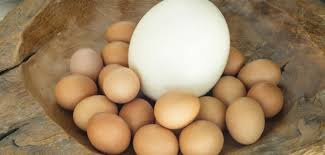
\includegraphics[width=.5\textwidth]{laRepro/oeuf.jpg}	
			\caption{Exemple de grappe d'oeufs de rainettes.}%
			\label{fig:autruche}
		\end{center}
=======
	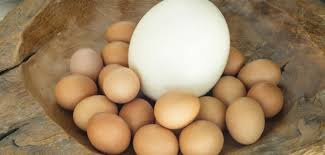
\includegraphics[width=.9\textwidth]{laRepro/oeuf.jpg}	
	\end{center}
	\caption{Exemple de grappe d'oeufs de rainettes.}%
	\label{fig:autruche}%
>>>>>>> 9c1c91cf300d3ed68f23f2e076351a9ee57079a7
\end{figure}

Il existe des périodes sensibles du développement, pendant lesquelles peuvent se développer des malformations embryonnaires graves : moins de 1 des oeufs fécondés parviennent à l’âge adulte
	

	\section*{Fables}
		\begin{enumerate}
			\item La Grenouille qui veut se faire aussi grosse que le Bœuf (Livre I, fable III),
			\item Les deux Taureaux et une Grenouille (Livre II, fable IV)
			\item Le Lièvre et les Grenouilles (Livre II, fable XIV)
			\item Les Grenouilles qui demandent un Roi (Livre III, fable IV)
			\item La Grenouille et le Rat (Livre IV, Fable XI)
			\item Le Soleil et les Grenouilles (Livre VI, fable XII)
		\end{enumerate}
	
	

	\section*{Fables}
		\begin{enumerate}
			\item La Grenouille qui veut se faire aussi grosse que le Bœuf (Livre I, fable III),
			\item Les deux Taureaux et une Grenouille (Livre II, fable IV)
			\item Le Lièvre et les Grenouilles (Livre II, fable XIV)
			\item Les Grenouilles qui demandent un Roi (Livre III, fable IV)
			\item La Grenouille et le Rat (Livre IV, Fable XI)
			\item Le Soleil et les Grenouilles (Livre VI, fable XII)
		\end{enumerate}

	
\section{Usage culinaire (mais perso, moi j'aime pas)}

Toutes les grenouilles ne sont pas comestibles. Certaines espèces sont même toxiques et d'autres sont des espèces menacées de disparition dont les populations sont désormais protégées.

En cuisine française, ce sont les cuisses qui sont consommées. Les Français ont la réputation mondiale d'être des mangeurs de grenouilles, ce qui leur a valu leur surnom anglais de froggies, frog signifiant grenouille en anglais. Ainsi, on appelle $\ll$ Vallée des grenouilles $\gg$ un quartier de Londres, peuplé de beaucoup de Français.
En Italie les Français sont parfois appelés les mangiarane, c'est-à-dire les $\ll$ mangeurs de grenouilles $\gg$.

Traditionnellement, il s'agissait d'espèces locales, comme les grenouilles rousses (Rana temporaria) et vertes (Rana esculenta) désormais protégées à l'état sauvage en France, mais encore disponibles dans de rares élevages agréés. Elles ont été remplacées par des grenouilles asiatiques : Rana tigrina, Rana crassa et Rana catesbeiana quand elles sont surgelées et Rana ridibunda pour les importations vivantes12. D'autres pays d'Europe ou les États-Unis consomment également ces grenouilles d'importation.

Les autochtones au Cameroun mangent couramment Trichobatrachus robustus : chassé avec de longues lances, des machettes, et même parfois des armes à feu pour éviter ses griffes rétractiles, il finit alors au menu, rôti (entier)14. Dans les monts Rumpi, zone protégée à l'ouest du Cameroun, les autochtones en mangent les têtards, qui seraient assez gros.

\begin{figure}
	\begin{center}
		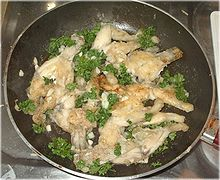
\includegraphics[scale=1]{cuisine/miam.JPG}
			\caption{Cuisses de grenouilles}
			\label{fig:gre}
	\end{center}
\end{figure}
				
\end{document}